\documentclass[format=acmsmall, review=false, screen=true]{acmart}

\usepackage{booktabs} % For formal tables

\usepackage[ruled]{algorithm2e} % For algorithms
\renewcommand{\algorithmcfname}{ALGORITHM}
\SetAlFnt{\small}
\SetAlCapFnt{\small}
\SetAlCapNameFnt{\small}
\SetAlCapHSkip{0pt}
\IncMargin{-\parindent}


% Metadata Information


% Copyright
%\setcopyright{acmcopyright}
%\setcopyright{acmlicensed}
%\setcopyright{rightsretained}
%\setcopyright{usgov}
%\setcopyright{usgovmixed}
%\setcopyright{cagov}
%\setcopyrightmode{relax}



% Paper history
%\received{February 2007}
%\received[revised]{March 2009}
%\received[accepted]{June 2009}
% Document starts
\begin{document}
% Title portion. Note the short title for running heads 
\title[Plane Sense]{Plane Sense \newline A 3D Sound Based Airplane Navigation Tool}

\author{Matthew Bregg}
\affiliation{%
  \institution{University of Florida}
}
\author{Nicolas Fry}
\affiliation{%
  \institution{University of Florida}
}
\author{Taariq Imami}
\affiliation{%
  \institution{University of Florida}
}
\author{DJ Meyers}
\affiliation{%
  \institution{University of Florida}
}

\begin{abstract}
  Inbsert abstract here
\end{abstract}



% We no longer use \terms command
%\terms{Design, Algorithms, Performance}

\keywords{3D Audio, Flight, Plane, Safety, Sound}


\maketitle

% The default list of authors is too long for headers}
\renewcommand{\shortauthors}{M. Bregg T. Imami D. Meyers N. Fry}

% \cite{Akyildiz-02, Harvard-01,CROSSBOW} and smart homes
\section{Introduction}
\paragraph{}
PlaneSense's target user population is within the scope of private aviation, airline transportation, and commercial aviation. Pilots, flight engineers, and all patrons of the cockpit are encouraged to utilize PlaneSense's technology that aims make the sky safe with minimal cost.  Between 2006 and 2015, 165 people died as a result of in-air collisions between airplanes \cite{Boeing}.  This number does not account for planes that lose control or crash while trying to avoid an in-air collision, such as the 2012 case of two planes approaching the runway at the same time, leading to one crashing \cite{brevard}.  While 165 deaths is only about 5\% of the total number of airplane-related deaths in this time period, these types of accidents can be avoided by providing pilots with better tools to be made aware of nearby aircraft.  All pilots should have access to a cheap, safe tool that will give them a quick, intuitive, and accurate survey of their immediate airspace, whether the pilot is flying small private planes or passenger laden commercial flights.


\paragraph{}
Currently, the onboard systems for detecting nearby planes are good; however, they tend to have some systemic flaws that can easily influence an accident. The current solutions range from simply looking outside, utilizing a ground radar with communication to the pilot, and costly, advanced systems like the \textit{Garmin G1000} \cite{Garmin}. Similar to earthbound vehicles, pilots looking at their instrument cluster are less likely to be aware of their surrounding. The easiest example to relate it to is texting and driving. Pilots will lose situational awareness and the risk of an accident will grow exponentially.


\paragraph{}
The most obvious way for a pilot to know that there are other planes close to them is to simply look out their windows, but this has its drawbacks.  Inclement weather, such as fog, can reduce visibility, and simply looking around will lead to blind-spots, much like in a car \cite{LAX06LA056B}. Sight can be quite useful, but is prone to error, and optical illusions, you might not see something small in the distance, even if looking right at it \cite{Ken}. 


\paragraph{}
Developed during World War II, radar was engineered by the United States Navy to detect aircraft and ships. Today, Radar's derivatives are used to track planes. The major downfall is that you would need to be in contact with someone on the ground in order to use it. Very rarely, do pilots have this equipped on the plane. The Garmin G1000 is a  glass cockpit solution which replaces instruments with electronics as well as an integrated gps with traffic. Although this is nice, it has three major downfalls. It will either need to be installed as a retrofitted device (for older aircraft) or purchased with a brand new aircraft. It also distracts the pilot when making complicated maneuvers such as going in for a landing.  

\paragraph{}


Using 3D audio, PlaneSense would present the flight crew with a "sixth sense" when it comes to plane safety.  Utilizing the flight crews' existing headsets, PlaneSense would present audio cues that can signify where other planes or obstructions are in relation to their aircraft. Unlike the other solutions, These auditory cues will appear to originate from the direction of nearby aircraft.  This would help increase a pilot's situational awareness, and decrease the cognitive load, for a safer, more pleasant, flight.  PlaneSense creates a natural way to alert pilots so that they can alter the plane's course or otherwise avoid a collision, by immediately and intuitively informing them of another plane's relative location. 




\paragraph{}
PlaneSense utilizes the  Automatic Dependent Surveillance-Broadcast system (ADS-B) to capture information about other aircraft in the vicinity.  Not every plane has a transponder equipped with ADS-B Out; however, by 2020 the Federal Aviation Administration will require them in all aircraft in US controlled airspace. This allows PlaneSense to detect all planes that are equipped with this technology.  Aircraft retrieve their position from onboard GPS systems and broadcast their location through the ADS-B out to other aircraft as well as ground stations. PlaneSense picks up the information from the towers, and creates a 3D mapping of nearby aircraft to be represented with 3D Audio.  \textit{Stratux}, an open-source aircraft traffic detection system, was used as a basis to interpret the information from the ADS-B.
PlaneSense will extend the features of \textit{Stratux}, and will provide some basic options,
such as volume, sounds to play, and maximum distance to detect.


\paragraph{}
Success was defined as making a pilot more situationally aware of their surroundings without increasing their cognitive workload.  For example, emulating the natural feeling of using GPS and creating the illusion of the sounds from other aircraft approaching or departing from the user would be considered a success.  The pilot would have an idea of where the other planes are, without wasting visual awareness on other instruments. By taking advantage of more of the pilot's senses, the pilot's overall capacity for awareness can be increased, thus, making flying more safe. In order to enable this technology to be widespread, and easily accessible, PlaneSense must allow integration into any stereo pilot headset. 


\paragraph{} 
PlaneSense's first major challenge was integration with the plane's existing systems. This problem was overcome by using the open source software, \textit{Stratux}.
By using open-source software to collect and analyze air traffic data, PlaneSense can be created and distributed at a much cheaper cost.
This enables more time to be spent on developing the 3D audio aspect of PlaneSense, rather than spent interpreting the format of ADS-B data.
The second major challenge was technical debugging, which could be performed in smart aircraft locally as well camping out by nearby airports.  PlaneSense is capable of detecting more airplanes than the pilot needs to know about, so a threshold needed to be set that would only alert the pilots of planes within a certain radius.  To avoid this issue, detecting one's own plane as appearing right above oneself, no planes within 100 feet of the PlaneSense device are reported.  This, among other aspects, would need to be fine tuned for different aircraft and operations. 

       \begin{figure}
         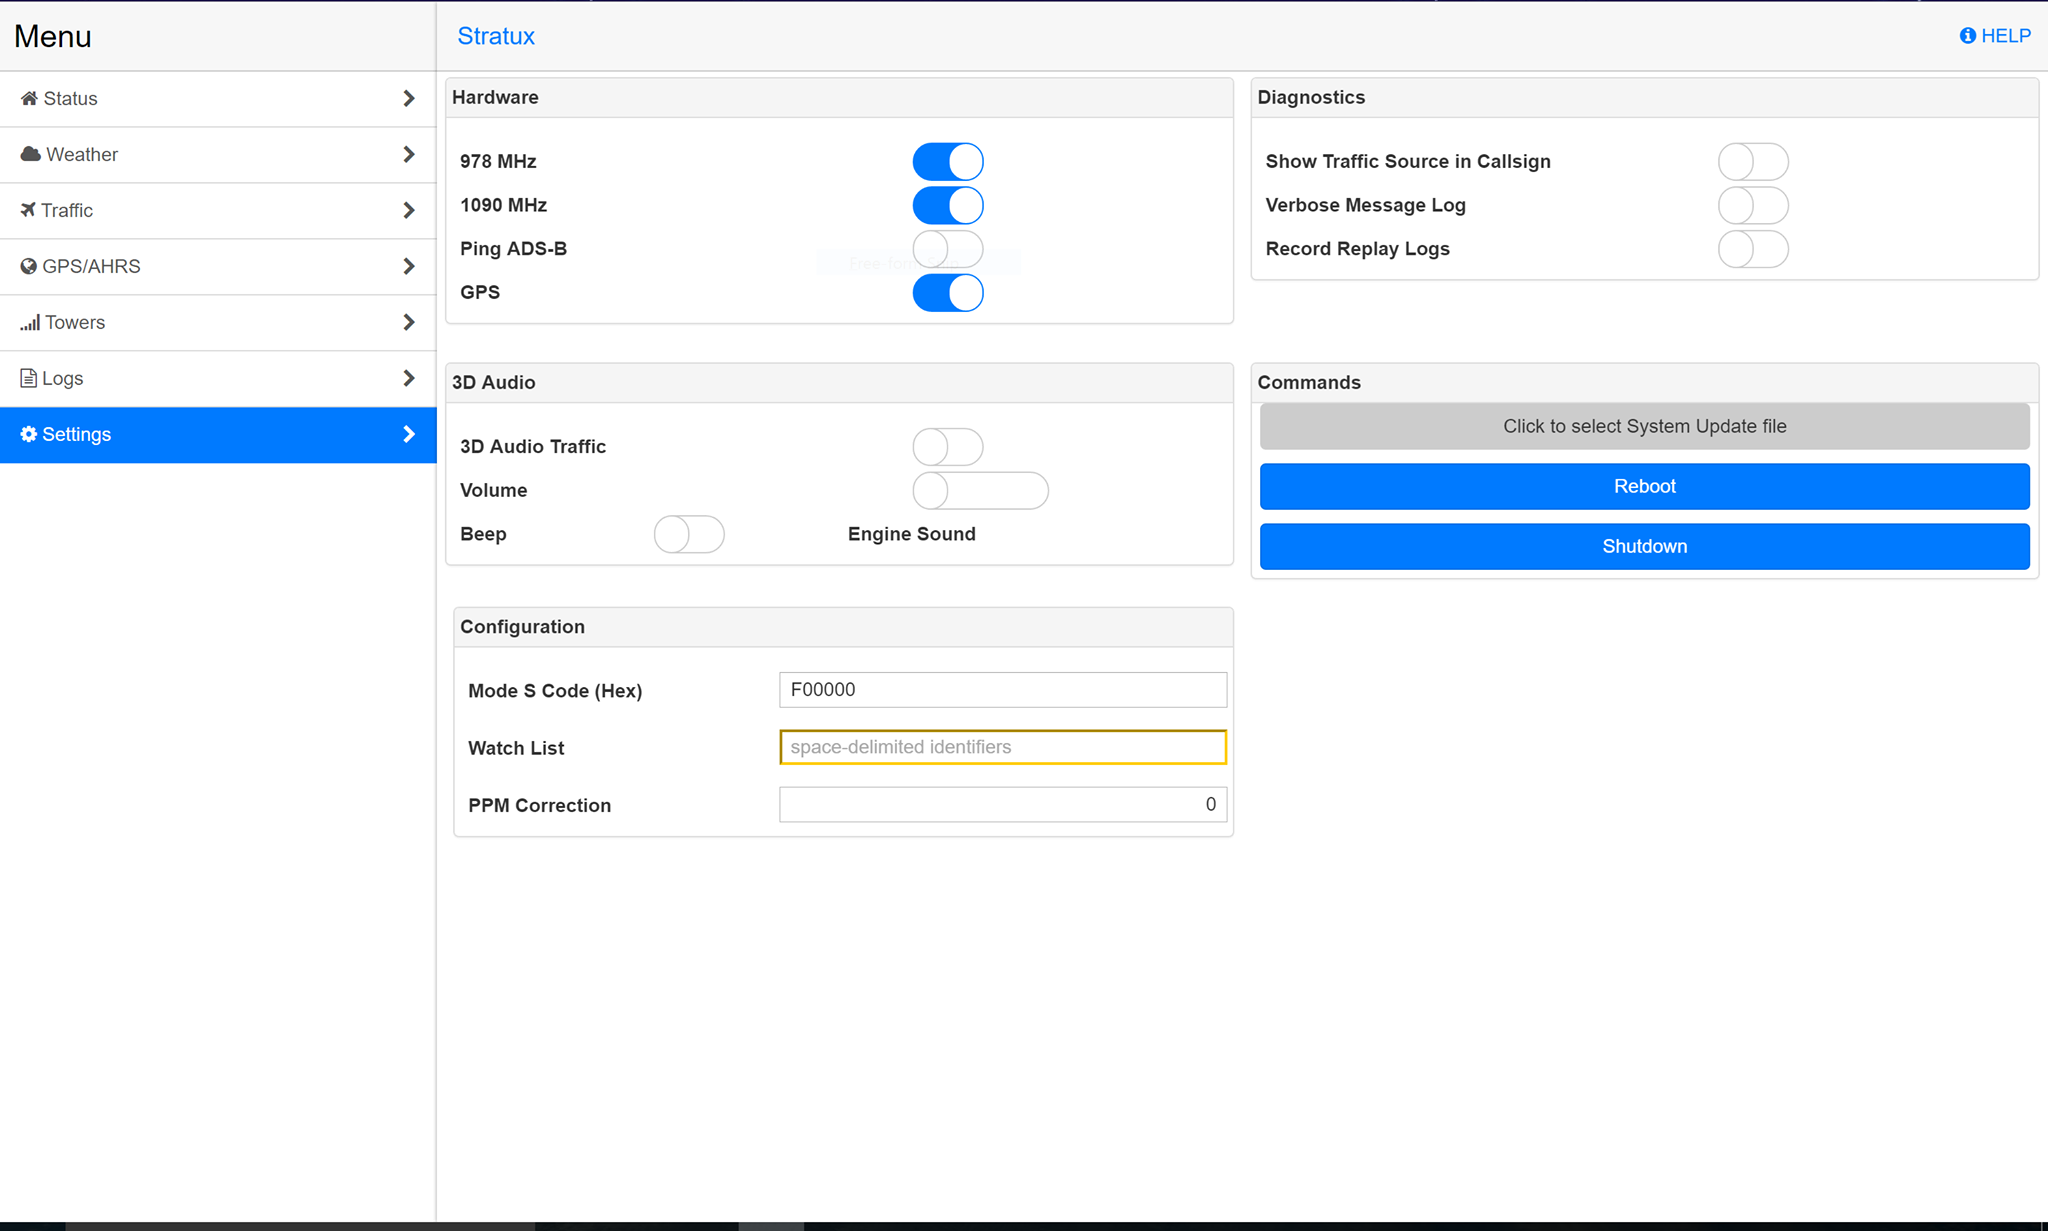
\includegraphics[width=\linewidth]{./sample_ui.png}
         \caption{A Mock-Up of how the PlaneSense UI will look. For the most part, it involves modifying a few preflight
           options, and then being left alone for the duration of the flight.}
         \label{fig:p1}
       \end{figure}

       
\section{Methods}


\paragraph{}
	In order to evaluate the effectiveness of PlaneSense, participants were gathered for a study and randomly divided into two groups of even size.  Both groups were instructed to remove the two and eight cards the from two decks of cards.  This task was chosen to give the participants a mentally stimulating task that they had to pay attention to so that they didn't miss a card, similar to the mental effort needed to maintain a steady course in an airplane.
	While the first group was separating cards from the deck, they were asked to look down at a mockup of a Stratux screen with traffic that a pilot may see while flying.  The participants' simulated flight path was due east.  These participants were asked to identify planes that were within 5 miles of them and to describe the plane's position relative to their own.

        \begin{figure}
          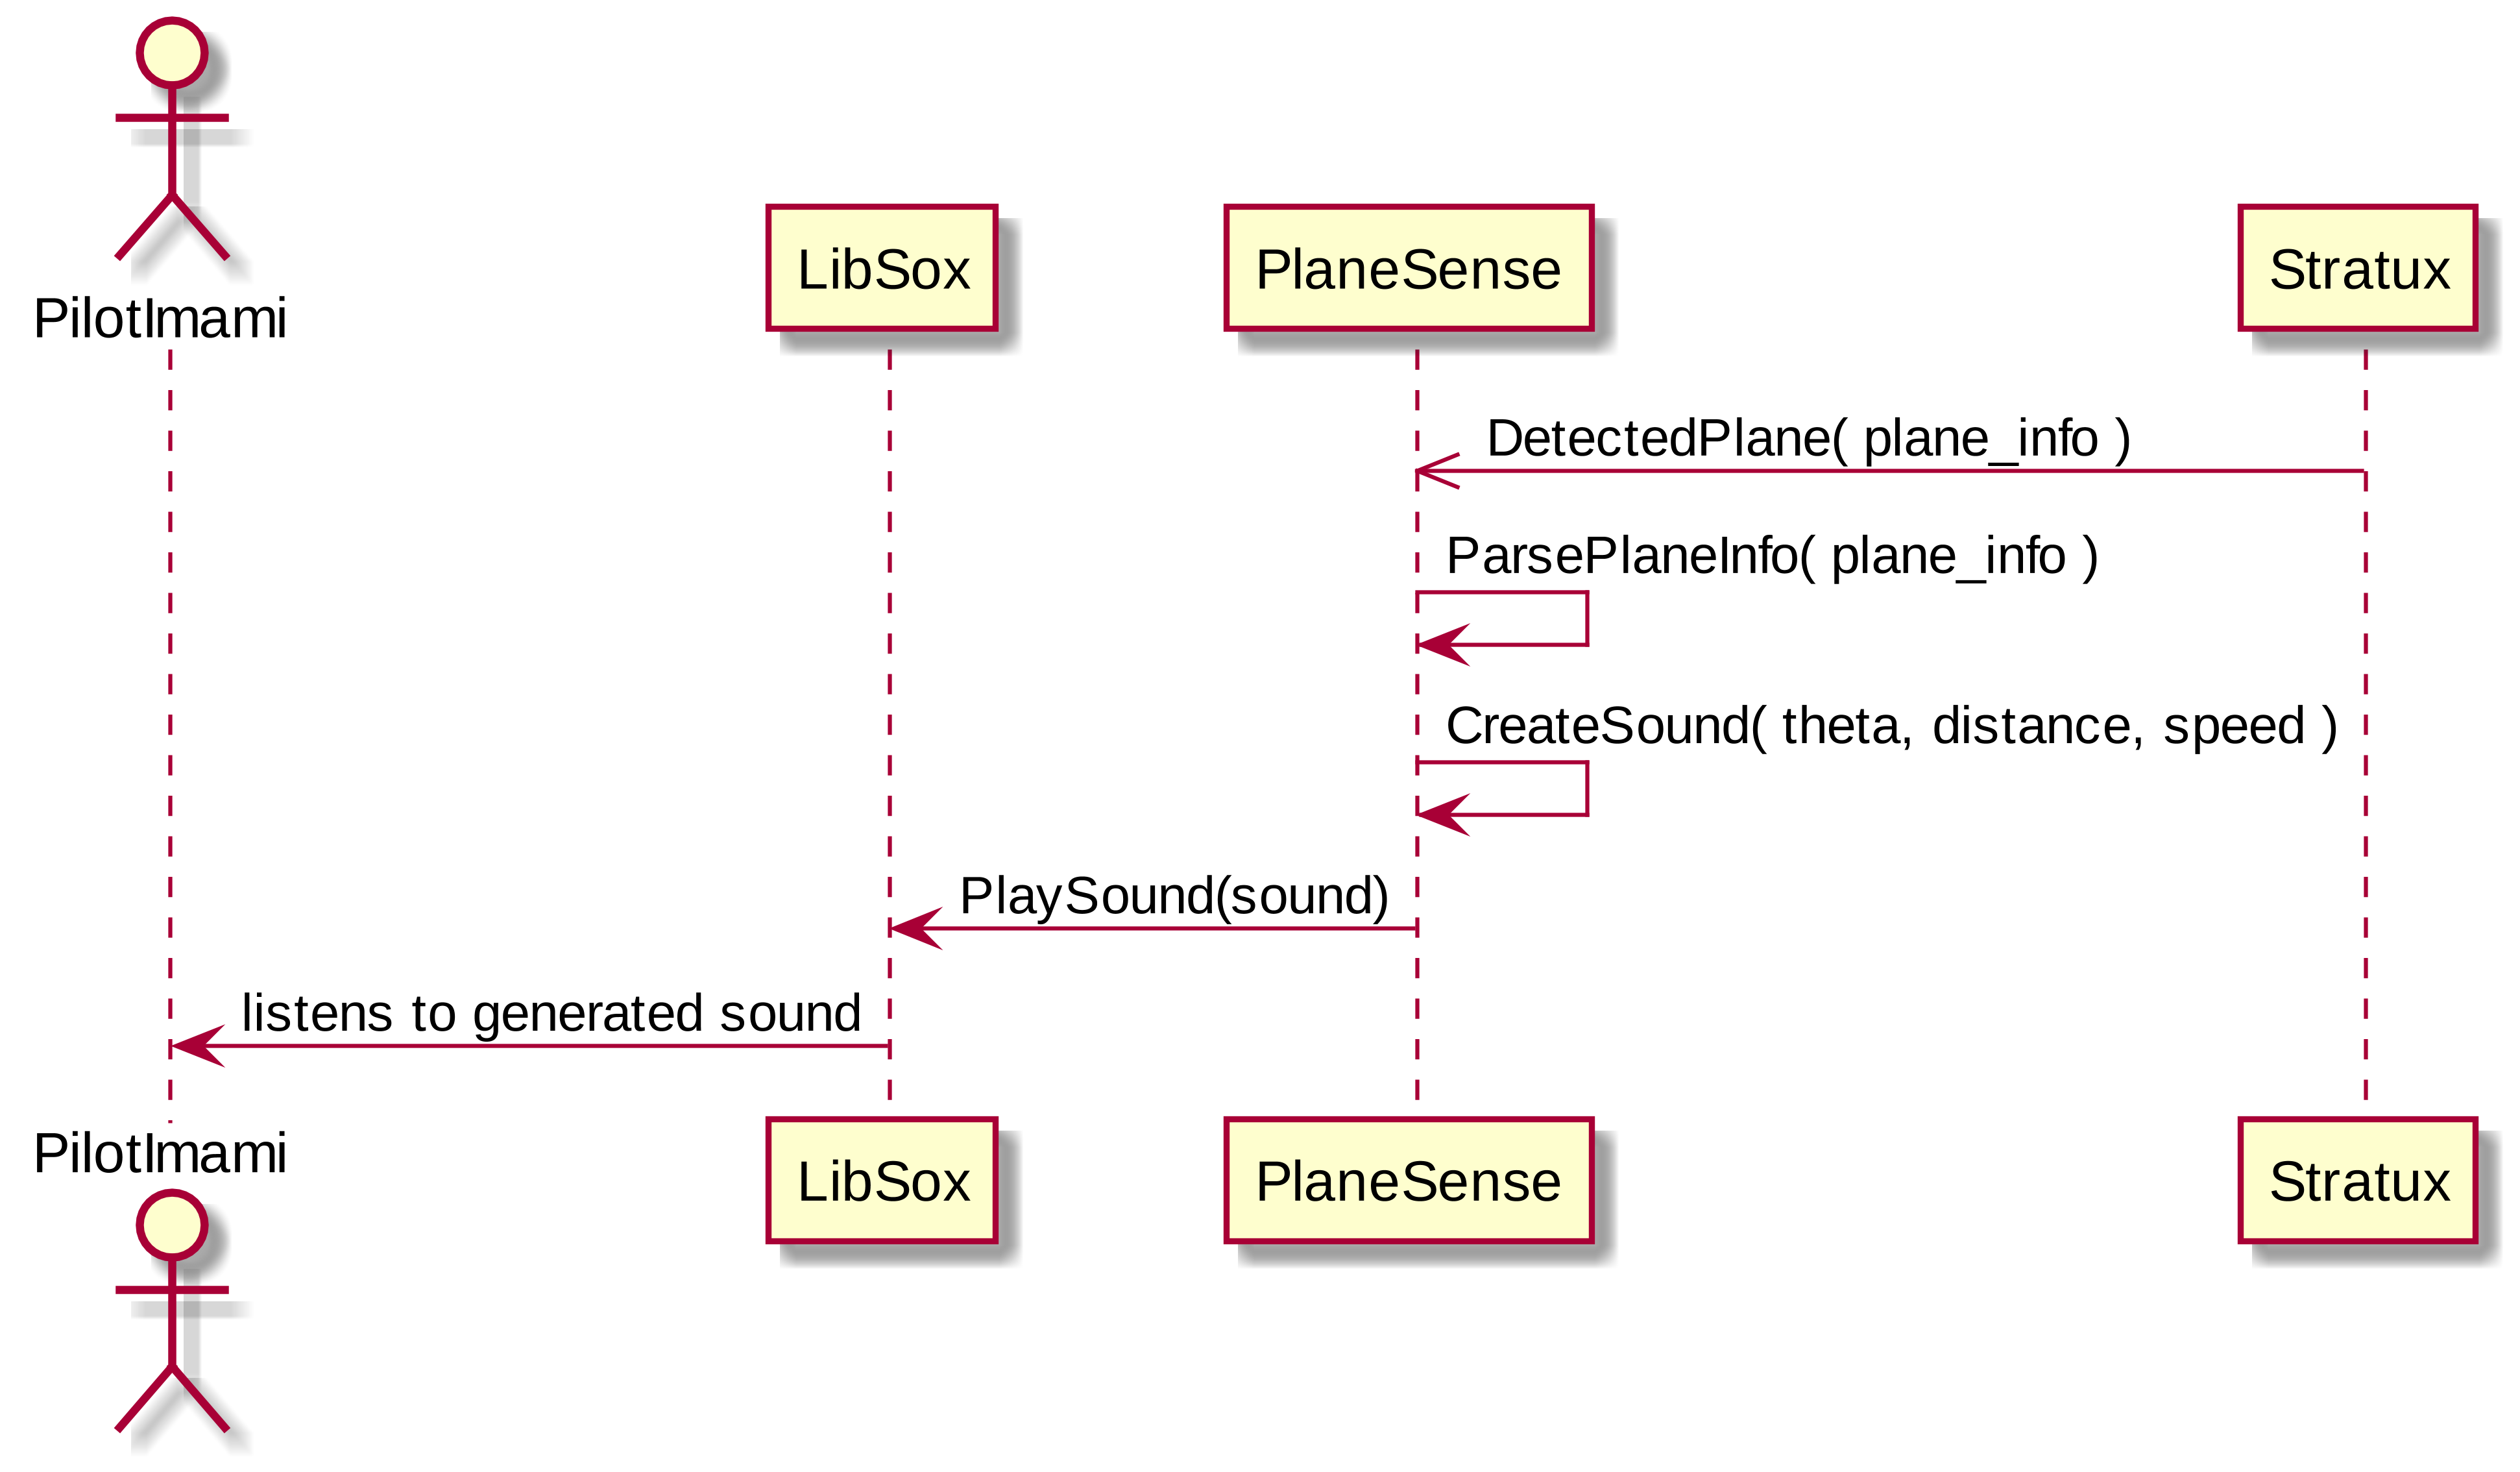
\includegraphics[width=\linewidth]{./sequence_diagram_for_plane_sense.png}
          \caption{System and Information Flow For Normal Use}
          \label{fig:n1}
        \end{figure}

        \begin{figure}
          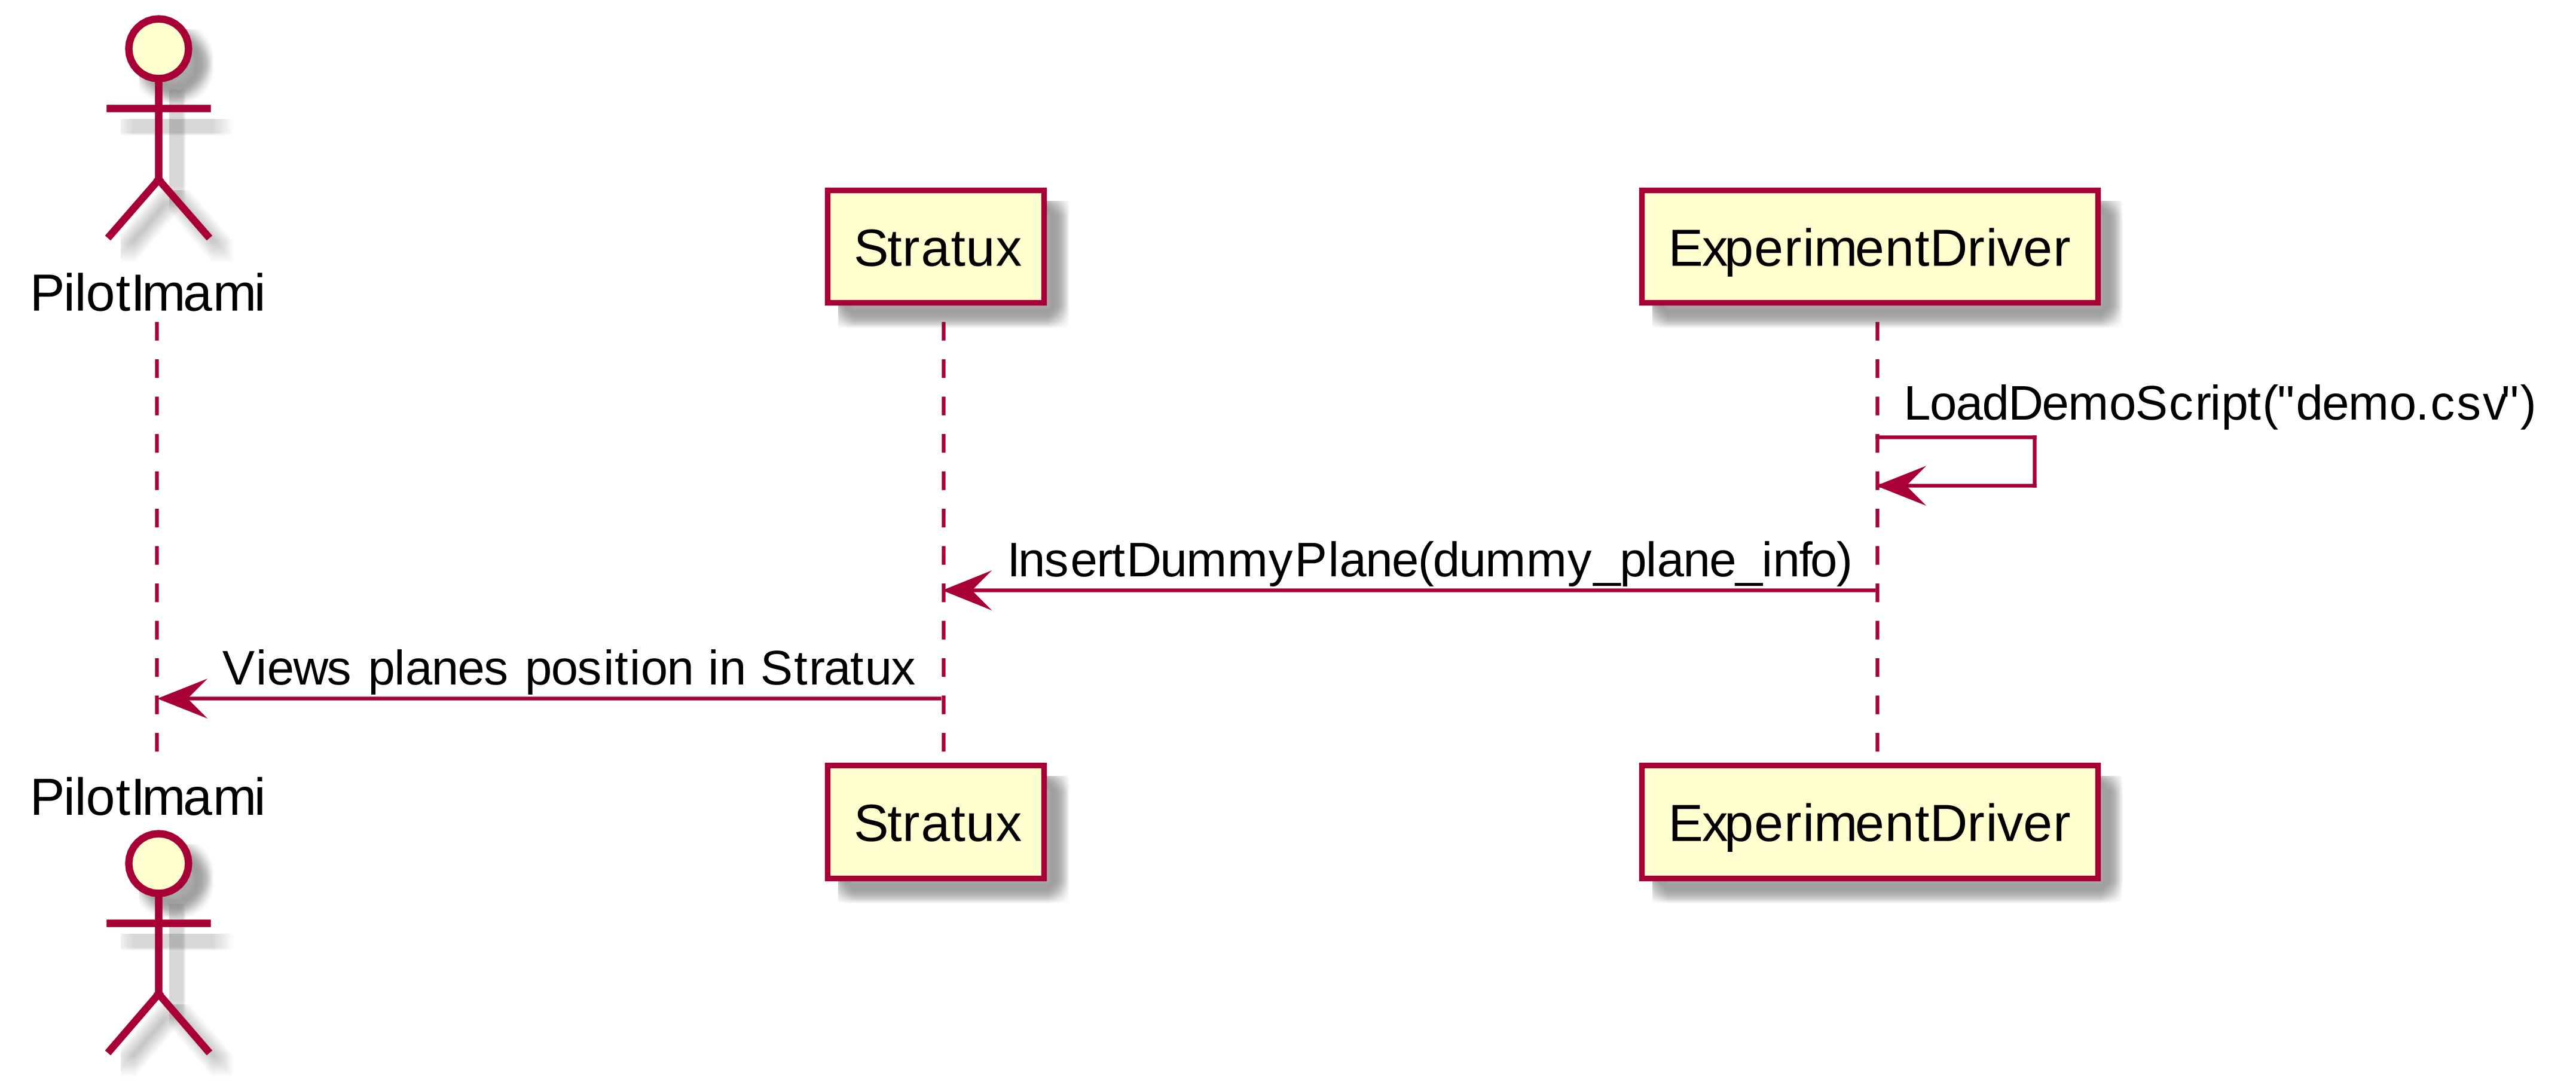
\includegraphics[width=\linewidth]{./sequence_diagram_for_experiment_g2.png}
          \caption{System and Information Flow For Group One}
          \label{fig:g1}
        \end{figure}

        \begin{figure}
         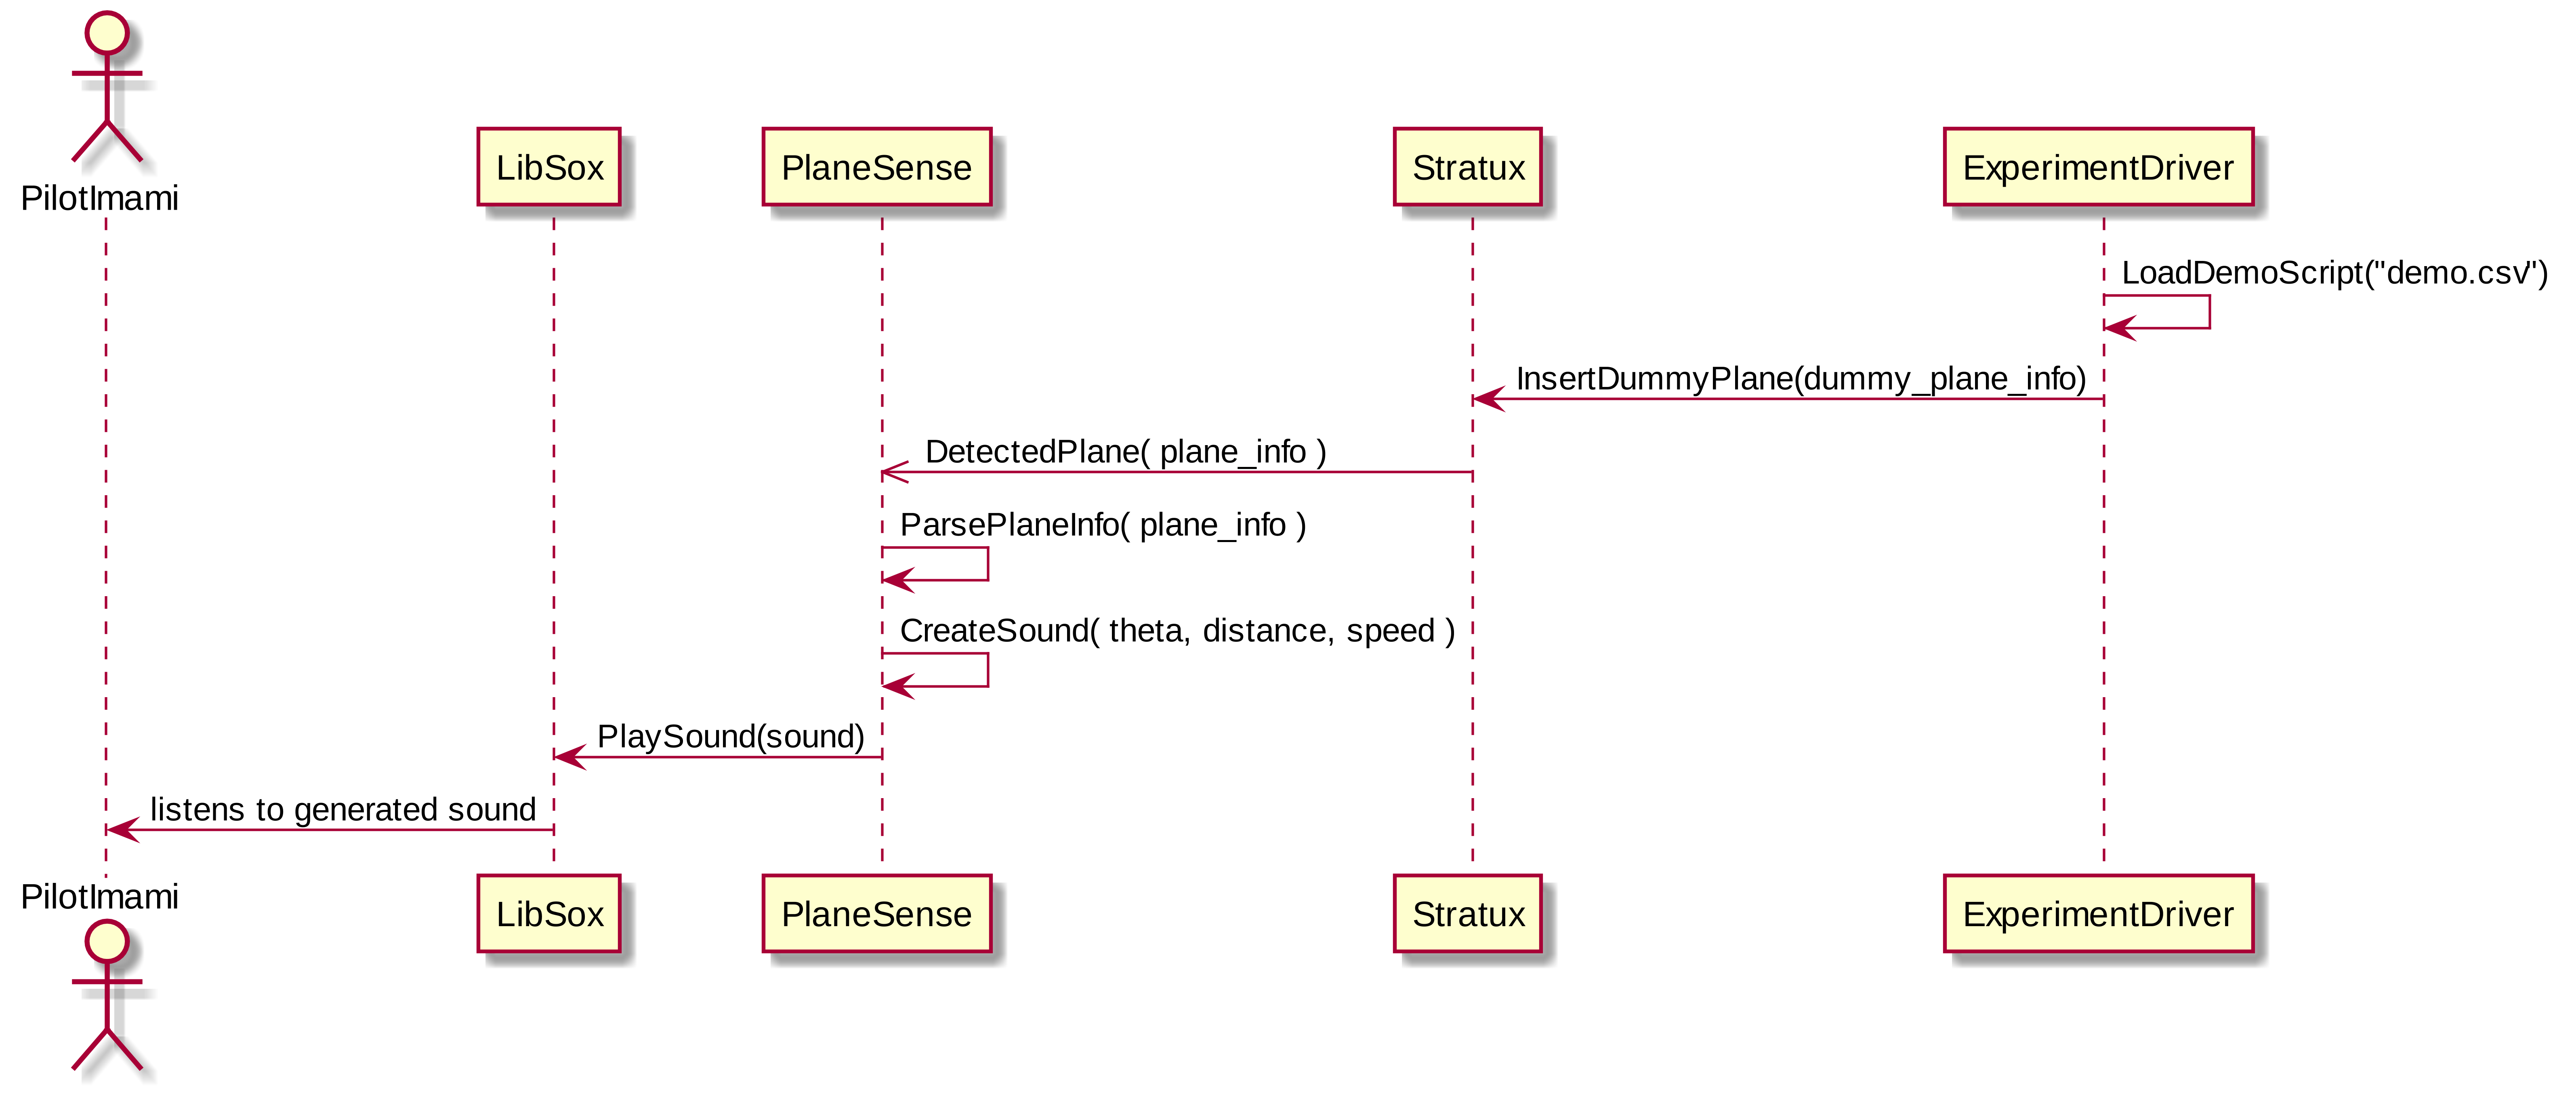
\includegraphics[width=\linewidth]{./sequence_diagram_for_experiment_g1.png}
         \caption{System and Information Flow For Group Two}
         \label{fig:g2}
       \end{figure}

While the second group was separating cards from the deck, they wore headphones that produced 3D audio cues.
These cues were beeping tones (C5 - 523.2 Hz) that were localized to appear to originate from the same relative positions of the planes that the first group had to identify, based on Head-Related Transfer Functions from the CIPIC HRTF Database.  The participants were asked to identify the planes' directions based only on audio cues.  They did not need to worry about distance, because PlaneSense only alerts users of planes within 5 miles.
Participants were timed with a stopwatch to measure how long it took them to identify 3 planes' locations while retrieving all 16 two and eight cards from two decks of cards.  Participants accuracy in sorting the cards was recorded to measure if trying to locate the planes decreased their ability to sort the cards.  The participants were also scored based on their ability to correctly locate other planes.  Participants then rated the mental effort needed to identify the planes while sorting cards via a google form.
% Bibliography
\bibliographystyle{ACM-Reference-Format}
\bibliography{sample-bibliography}

\end{document}
